% !TEX root = ../../main.tex

\section{Saved state} % (fold)
\label{sec:saved_state}

The \acrshort{api} also allows for an initialisation with a certain state passed in. This means that it's possible to save a state Object in a location, and then later restart the search from that data. 

This is useful for three major use cases. The first is \acrshort{url} synchronisation. For \acrshort{url} synchronisation the structure would be to first listen on every state change with {\tt .subscribe()}, and then asynchronously transform that to query parameters to set. If a user comes to a page with query parameters, a function to take in the query string and put out a state Object would then be called. After that point a new InstantSearch Core instance can be built with the {\tt preloadedState} parameter set in the constructor.

\begin{figure}[H]
  \centering
  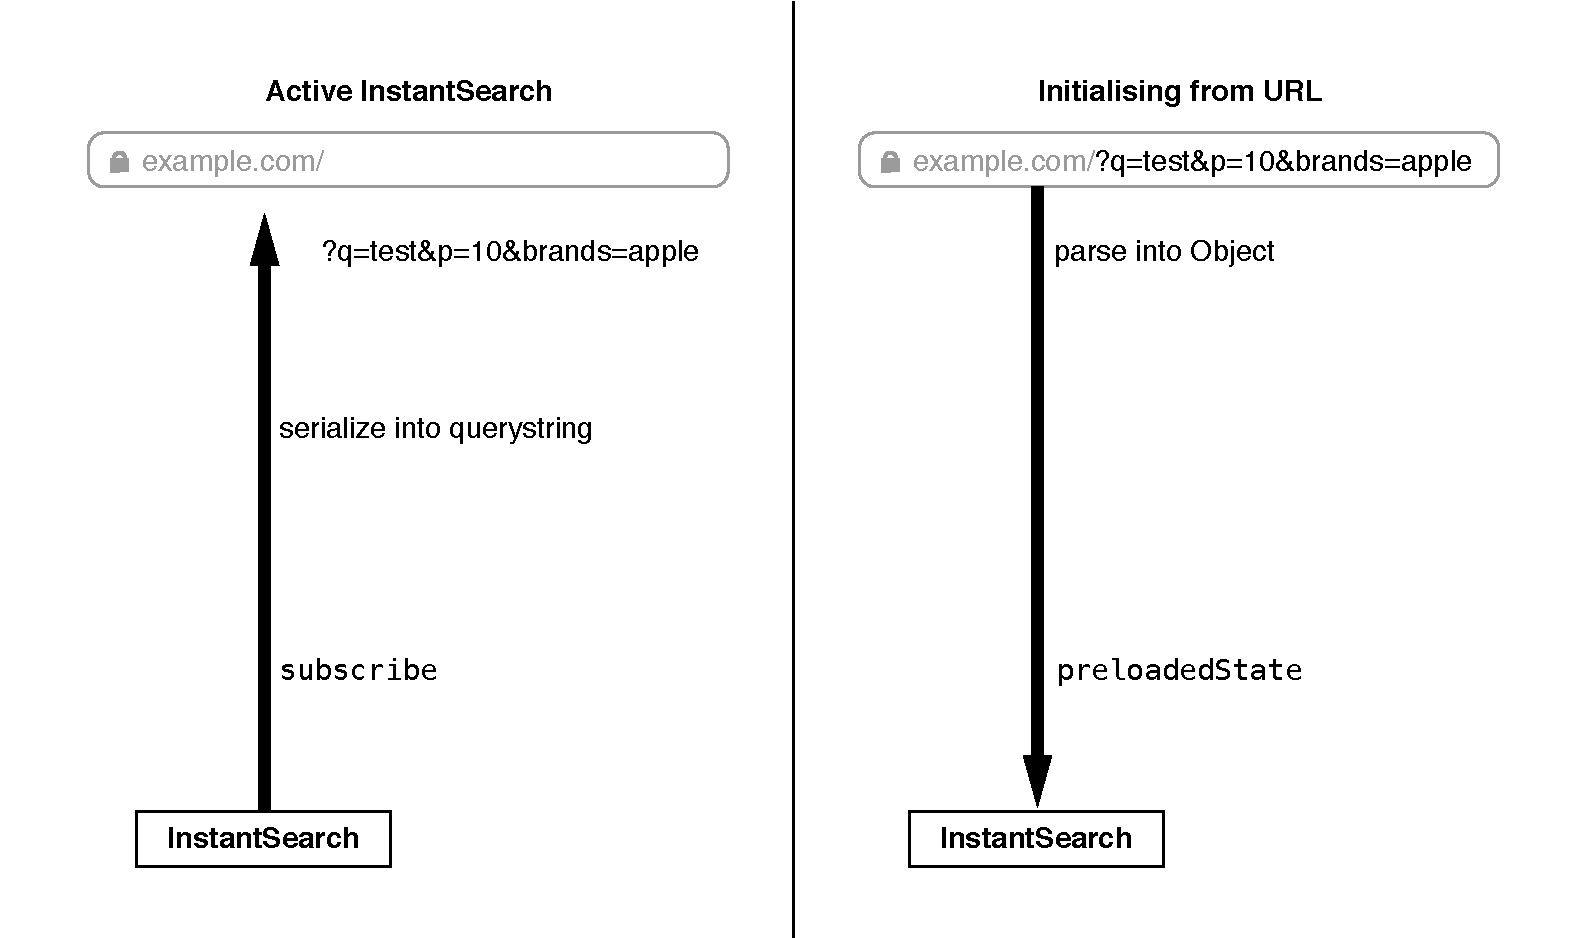
\includegraphics[width=0.8\textwidth]{../assets/is-core-url-sync.pdf}
  \caption{Synchronisation with the querystring using InstantSearch Core}
  \label{figure:is-core-url-sync}
\end{figure}

Similarly it is also possible to do that process with a different medium than query parameters, for example {\tt localStorage}. For that reason this process is left over to the user, possibly with other small packages dealing with browser inconsistencies on top of it. 

This pattern is also useful for when \acrfull{ssr} is implemented. When implementing \acrlong{ssr}, instead of sending an empty \acrshort{dom} and JavaScript to the browser, the first render will be done on the server instead. After that step, the client-side rendering will take over --- also called hydrating --- the \acrshort{dom} in order for it to become interactive. When dealing with asynchronously fetching data --- which is the case when using the Algolia \acrshort{api} --- not the first render will be sent to the client, but rather the first render after a fetch has been completed.

To allow for this pattern, the following steps need to be executed:

\begin{enumerate}
  \item execute the InstantSearch function once
  \item render the output as \acrshort{html}
  \item also output the state Object in a global Object in a script tag
  \item send that \acrshort{html} to the client
  \item start the InstantSearch instance frontend with {\tt window.PRELOADED\_STATE} as {\tt preloadedState}
\end{enumerate}

Having a hook to define state before rendering will allow one to create each refinement on the fly. This means that, while the \acrshort{api} request goes through on the server once, just the needed resources will be fetched a second time from the client-side application. 

\begin{figure}[H]
  \centering
  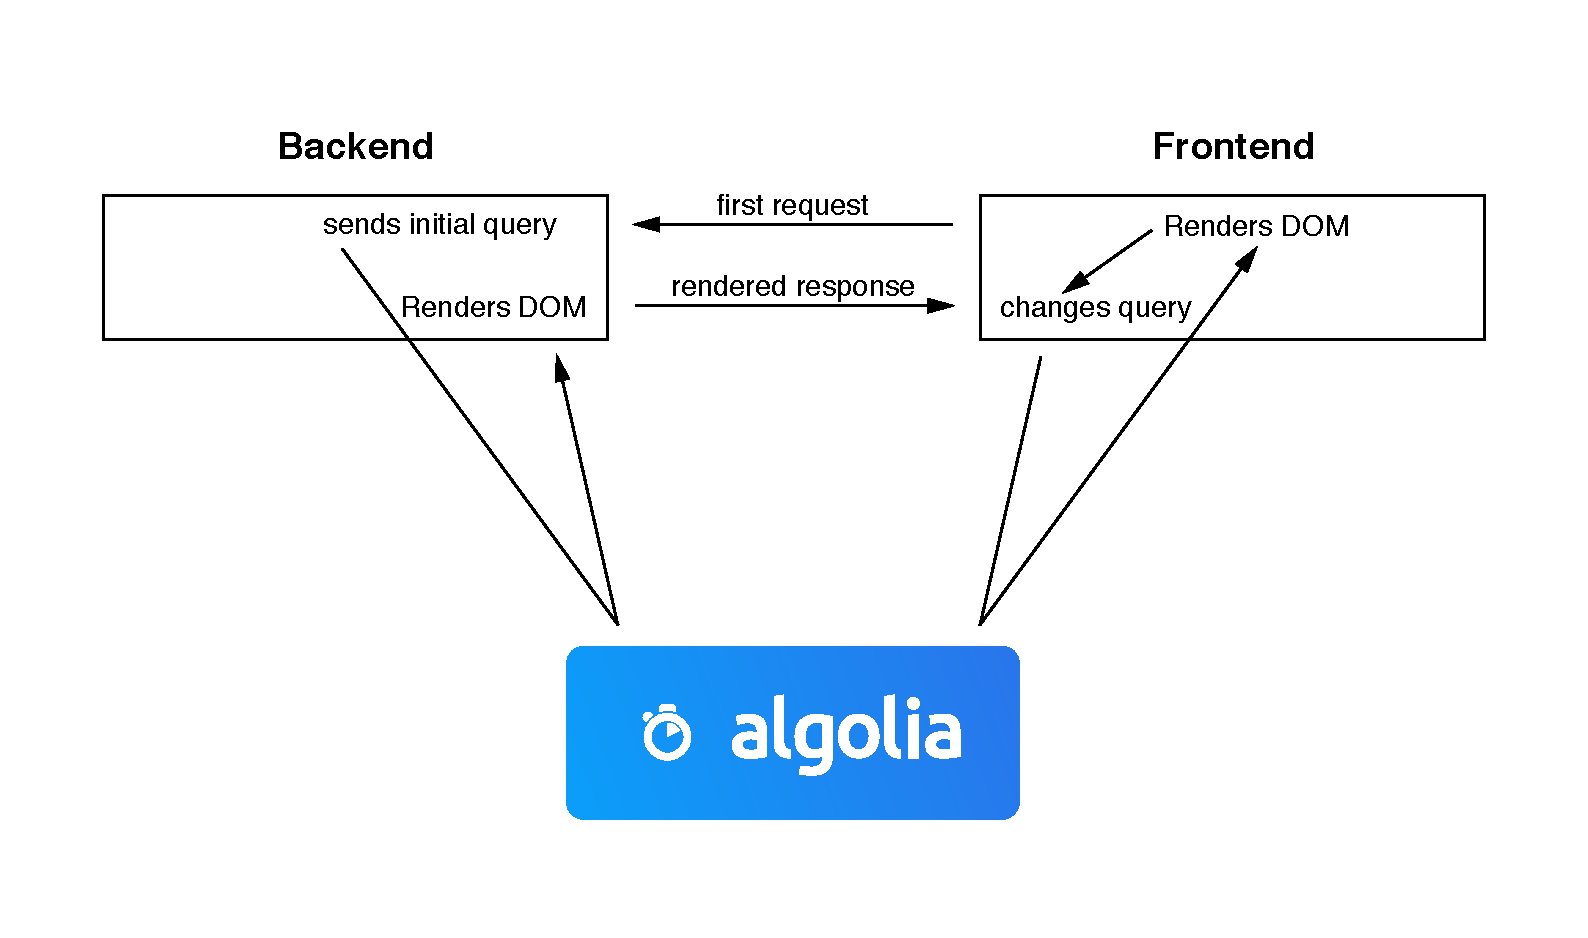
\includegraphics[height=0.4\textheight]{../assets/is-core-ssr.pdf}
  \caption{Server Side Rendering with InstantSearch Core}
  \label{figure:is-core-ssr}
\end{figure}

% section saved_state (end)
